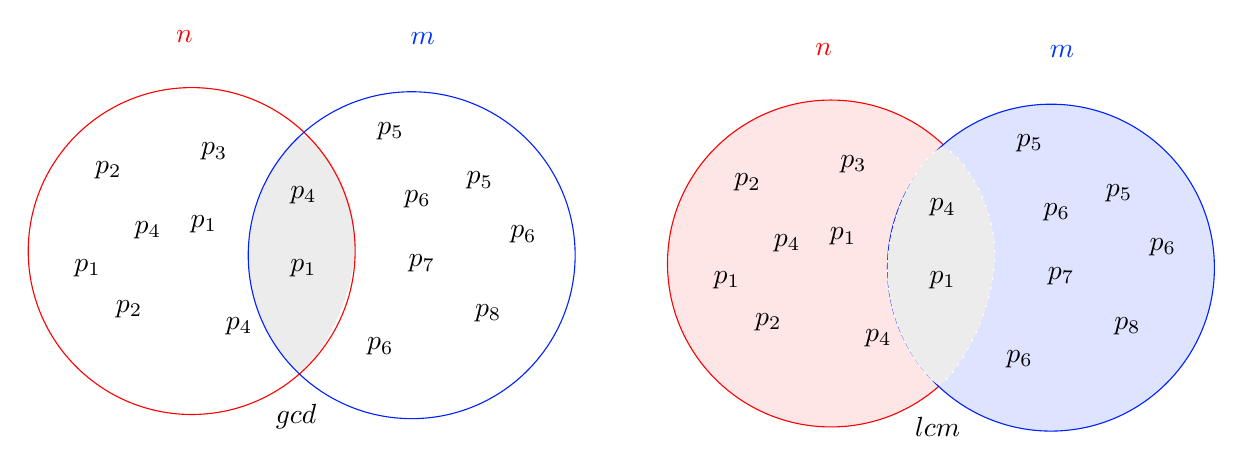
\begin{tikzpicture}[x=0.75pt,y=0.75pt,yscale=-1,xscale=1]
%uncomment if require: \path (0,300); %set diagram left start at 0, and has height of 300

%Shape: Polygon Curved [id:ds11586985302725228] 
\draw  [color={rgb, 255:red, 255; green, 255; blue, 255 }  ,draw opacity=1 ][fill={rgb, 255:red, 236; green, 236; blue, 236 }  ,fill opacity=1 ][dash pattern={on 0.84pt off 2.51pt}] (171.5,106) .. controls (165.5,106) and (145.5,131.5) .. (145,163.75) .. controls (144.5,196) and (165.5,219) .. (169.5,220) .. controls (173.5,221) and (194.5,192.5) .. (196.5,161.75) .. controls (198.5,131) and (177.5,106) .. (171.5,106) -- cycle ;
%Shape: Circle [id:dp8877599774135008] 
\draw  [color={rgb, 255:red, 255; green, 0; blue, 0 }  ,draw opacity=1 ] (39,161.75) .. controls (39,118.26) and (74.26,83) .. (117.75,83) .. controls (161.24,83) and (196.5,118.26) .. (196.5,161.75) .. controls (196.5,205.24) and (161.24,240.5) .. (117.75,240.5) .. controls (74.26,240.5) and (39,205.24) .. (39,161.75) -- cycle ;
%Shape: Circle [id:dp03762286895990197] 
\draw  [color={rgb, 255:red, 0; green, 33; blue, 255 }  ,draw opacity=1 ] (145,163.75) .. controls (145,120.26) and (180.26,85) .. (223.75,85) .. controls (267.24,85) and (302.5,120.26) .. (302.5,163.75) .. controls (302.5,207.24) and (267.24,242.5) .. (223.75,242.5) .. controls (180.26,242.5) and (145,207.24) .. (145,163.75) -- cycle ;
%Shape: Circle [id:dp7231634235092831] 
\draw  [color={rgb, 255:red, 255; green, 0; blue, 0 }  ,draw opacity=1 ][fill={rgb, 255:red, 255; green, 230; blue, 230 }  ,fill opacity=1 ] (347,167.75) .. controls (347,124.26) and (382.26,89) .. (425.75,89) .. controls (469.24,89) and (504.5,124.26) .. (504.5,167.75) .. controls (504.5,211.24) and (469.24,246.5) .. (425.75,246.5) .. controls (382.26,246.5) and (347,211.24) .. (347,167.75) -- cycle ;
%Shape: Circle [id:dp8270422939428064] 
\draw  [color={rgb, 255:red, 0; green, 33; blue, 255 }  ,draw opacity=1 ][fill={rgb, 255:red, 222; green, 228; blue, 255 }  ,fill opacity=1 ] (453,169.75) .. controls (453,126.26) and (488.26,91) .. (531.75,91) .. controls (575.24,91) and (610.5,126.26) .. (610.5,169.75) .. controls (610.5,213.24) and (575.24,248.5) .. (531.75,248.5) .. controls (488.26,248.5) and (453,213.24) .. (453,169.75) -- cycle ;
%Shape: Polygon Curved [id:ds17068028777126332] 
\draw  [color={rgb, 255:red, 255; green, 255; blue, 255 }  ,draw opacity=1 ][fill={rgb, 255:red, 236; green, 236; blue, 236 }  ,fill opacity=1 ][dash pattern={on 0.84pt off 2.51pt}] (479.5,112) .. controls (473.5,112) and (453.5,137.5) .. (453,169.75) .. controls (452.5,202) and (473.5,225) .. (477.5,226) .. controls (481.5,227) and (502.5,198.5) .. (504.5,167.75) .. controls (506.5,137) and (485.5,112) .. (479.5,112) -- cycle ;

% Text Node
\draw (109,54.4) node [anchor=north west][inner sep=0.75pt]  [color={rgb, 255:red, 255; green, 0; blue, 0 }  ,opacity=1 ]  {$n$};
% Text Node
\draw (116,143.4) node [anchor=north west][inner sep=0.75pt]    {$p_{1}$};
% Text Node
\draw (164,164.4) node [anchor=north west][inner sep=0.75pt]    {$p_{1}$};
% Text Node
\draw (60,164.4) node [anchor=north west][inner sep=0.75pt]    {$p_{1}$};
% Text Node
\draw (80,184.4) node [anchor=north west][inner sep=0.75pt]    {$p_{2}$};
% Text Node
\draw (70,117.4) node [anchor=north west][inner sep=0.75pt]    {$p_{2}$};
% Text Node
\draw (121,108.4) node [anchor=north west][inner sep=0.75pt]    {$p_{3}$};
% Text Node
\draw (164,129.4) node [anchor=north west][inner sep=0.75pt]    {$p_{4}$};
% Text Node
\draw (89,146.4) node [anchor=north west][inner sep=0.75pt]    {$p_{4}$};
% Text Node
\draw (133,192.4) node [anchor=north west][inner sep=0.75pt]    {$p_{4}$};
% Text Node
\draw (222,55.4) node [anchor=north west][inner sep=0.75pt]  [color={rgb, 255:red, 0; green, 50; blue, 255 }  ,opacity=1 ]  {$m$};
% Text Node
\draw (157,234.4) node [anchor=north west][inner sep=0.75pt]    {$\text{gcd}$};
% Text Node
\draw (206,98.4) node [anchor=north west][inner sep=0.75pt]    {$p_{5}$};
% Text Node
\draw (249,122.4) node [anchor=north west][inner sep=0.75pt]    {$p_{5}$};
% Text Node
\draw (201,202.4) node [anchor=north west][inner sep=0.75pt]    {$p_{6}$};
% Text Node
\draw (270,148.4) node [anchor=north west][inner sep=0.75pt]    {$p_{6}$};
% Text Node
\draw (219,131.4) node [anchor=north west][inner sep=0.75pt]    {$p_{6}$};
% Text Node
\draw (221,162.4) node [anchor=north west][inner sep=0.75pt]    {$p_{7}$};
% Text Node
\draw (253,186.4) node [anchor=north west][inner sep=0.75pt]    {$p_{8}$};
% Text Node
\draw (417,60.4) node [anchor=north west][inner sep=0.75pt]  [color={rgb, 255:red, 255; green, 0; blue, 0 }  ,opacity=1 ]  {$n$};
% Text Node
\draw (424,149.4) node [anchor=north west][inner sep=0.75pt]    {$p_{1}$};
% Text Node
\draw (472,170.4) node [anchor=north west][inner sep=0.75pt]    {$p_{1}$};
% Text Node
\draw (368,170.4) node [anchor=north west][inner sep=0.75pt]    {$p_{1}$};
% Text Node
\draw (388,190.4) node [anchor=north west][inner sep=0.75pt]    {$p_{2}$};
% Text Node
\draw (378,123.4) node [anchor=north west][inner sep=0.75pt]    {$p_{2}$};
% Text Node
\draw (429,114.4) node [anchor=north west][inner sep=0.75pt]    {$p_{3}$};
% Text Node
\draw (472,135.4) node [anchor=north west][inner sep=0.75pt]    {$p_{4}$};
% Text Node
\draw (397,152.4) node [anchor=north west][inner sep=0.75pt]    {$p_{4}$};
% Text Node
\draw (441,198.4) node [anchor=north west][inner sep=0.75pt]    {$p_{4}$};
% Text Node
\draw (530,61.4) node [anchor=north west][inner sep=0.75pt]  [color={rgb, 255:red, 0; green, 50; blue, 255 }  ,opacity=1 ]  {$m$};
% Text Node
\draw (465,240.4) node [anchor=north west][inner sep=0.75pt]    {$\text{lcm}$};
% Text Node
\draw (514,104.4) node [anchor=north west][inner sep=0.75pt]    {$p_{5}$};
% Text Node
\draw (557,128.4) node [anchor=north west][inner sep=0.75pt]    {$p_{5}$};
% Text Node
\draw (509,208.4) node [anchor=north west][inner sep=0.75pt]    {$p_{6}$};
% Text Node
\draw (578,154.4) node [anchor=north west][inner sep=0.75pt]    {$p_{6}$};
% Text Node
\draw (527,137.4) node [anchor=north west][inner sep=0.75pt]    {$p_{6}$};
% Text Node
\draw (529,168.4) node [anchor=north west][inner sep=0.75pt]    {$p_{7}$};
% Text Node
\draw (561,192.4) node [anchor=north west][inner sep=0.75pt]    {$p_{8}$};


\end{tikzpicture}
